%\thispagestyle{myheadings}
\newpage
\section{Keynote Speaker: Diyi Yang}
\setheaders{Keynote Speaker}{\daydateyear}
\index{Yang, Diyi}

\begin{center}
{\bfseries\Large Human Centered NLP for Positive Impact} \\
\vspace{1.0em}
{\large\bf Diyi Yang} \\
Stanford University

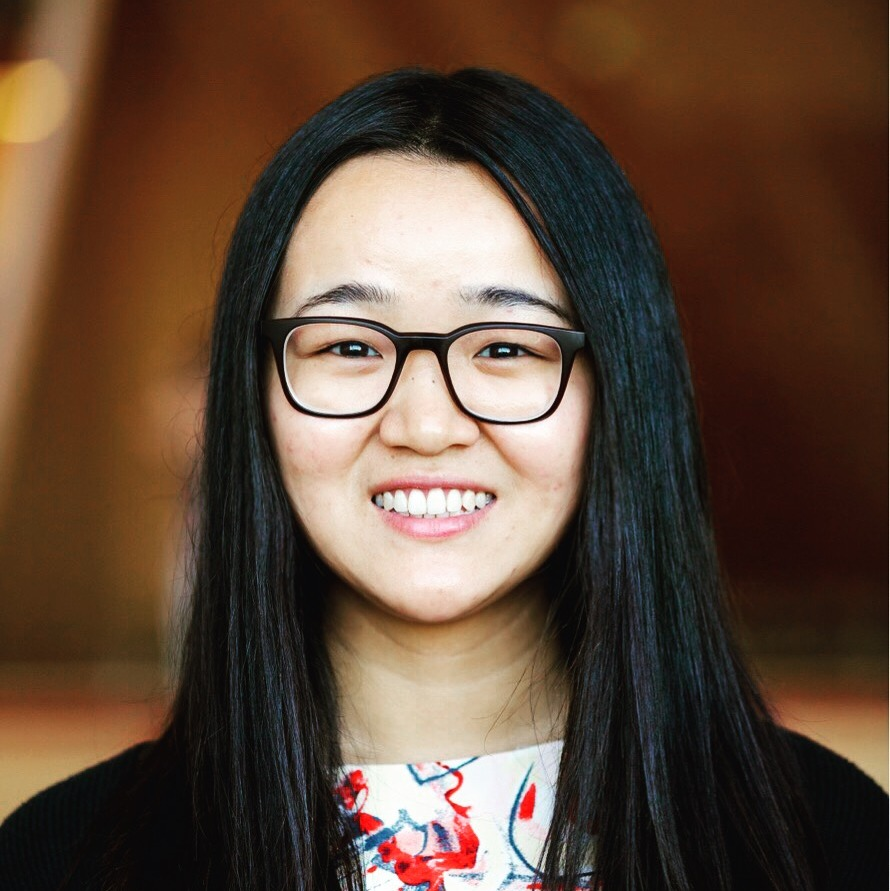
\includegraphics[width=0.4\linewidth]{content/mexican_nlp/diyi.jpeg}

\textbf{\daydateyear{}, 09:00--10:00 CST}\\
\textbf{Do\~na Adelita}
\end{center}

\noindent
{\bfseries Abstract:}
Large language models have revolutionized the way humans interact with AI systems, transforming a wide range of fields and disciplines. However, there is a growing amount of evidence and concern about the negative aspects of NLP systems such as biases and the lack of input from users. How can we build NLP systems that are more aware of human factors? In this talk, we will present two case studies on how human-centered design can be leveraged to build responsible NLP applications. The first one presents a participatory design approach to develop dialect-inclusive language tools and adaptation techniques for low-resourced language and dialect. The second part looks at social skill training with LLMs by demonstrating how we use LLMs to teach conflict resolution skills through simulated practice. We conclude by discussing how human-AI interaction via LLMs can empower individuals and foster positive change.

\vspace{1em}

{\bfseries Biography:}
Diyi Yang is an assistant professor in the Computer Science Department at Stanford University, also affiliated with the Stanford NLP Group, Stanford HCI Group and Stanford Human Centered AI Institute. Her research focuses on human-centered natural language processing and computational social science. She is a recipient of IEEE “AI 10 to Watch” (2020), Microsoft Research Faculty Fellowship (2021), NSF CAREER Award (2022), an ONR Young Investigator Award (2023), and a Sloan Research Fellowship (2024). Her work has received multiple paper awards or nominations at top NLP and HCI conferences, (e.g., Best Paper Honorable Mention at ICWSM 2016, Best Paper Honorable Mention at SIGCHI 2019, and Outstanding Paper at ACL 2022).

\newpage
